\documentclass[12pt]{article}

% Packages
\usepackage{amsmath}
\usepackage{amsfonts}
\usepackage{graphicx}
\usepackage{hyperref}
\usepackage{subfigure}
\usepackage{appendix}
\usepackage{parskip}

\usepackage[backend=biber]{biblatex}
\addbibresource{references.bib}

% Graphics
\usepackage{tikz}
\usetikzlibrary{positioning, shapes.geometric}

% Title and Author
\title{A TypeScript Based Agent-based Disease Model}
\author{Heyan Zhu (Anson)\\
\footnotesize Mathmatics \& Computer Science Class\\
\footnotesize \texttt{heyan.zhu@ulink.cn}}
\date{\today}

\begin{document}

% Title Page
\maketitle

% Abstract
\begin{abstract}
This paper presents an agent-based model implemented in TypeScript, which simulates the spread of diseases. It compares this model with the SIR model.
\end{abstract}

% \newpage
% Main content
\newcommand{\md}{\mathrm{d}}

\section{Introduction}
An agent-based model is a computer simulation of the interaction of agents (people) that is used to predict and demonstrate the spread of diseases \cite{columbiaGeneral}. This paper presents a TypeScript-based agent-based model that can partially simulate the spread of disease.

The code of the model is available on GitHub \footnote{\url{https://github.com/Anson2251/camp-agent-base-model}}.

\subsection{Mathematics theory of spread of disease}
In the field of mathematics, there also exists a model known as the SIR model, which is a set of differential equations that describe the number of people who are susceptible ($S$, not infected), infected ($I$), and recovered ($R$, have recovered from the illness and are no longer susceptible to the same disease). The equations of the SIR model are as follows:

\begin{align}
    \frac{\md S}{\md t}&=-\beta S I\\
    \frac{\md I}{\md t}&=\beta S I-\gamma I\\
    \frac{\md R}{\md t}&=\gamma I
\end{align}

\begin{figure}[h]
	\begin{minipage}[h]{0.3\linewidth}
		\centering
		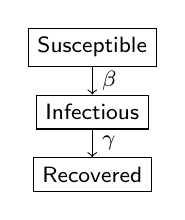
\begin{tikzpicture}[node distance=10pt]
    \tikzset{style={font=\sffamily\footnotesize}}
    \node[draw]                         (susceptible)   {Susceptible};
    \node[draw, below=of susceptible]    (infectious)    {Infectious};
    \node[draw, below=of infectious]     (recovered)     {Recovered};
    
    \draw[->] (susceptible)  -- node[right] {$\beta$} (infectious);
    \draw[->] (infectious) -- node[right] {$\gamma$} (recovered);
\end{tikzpicture}
        \caption{\scriptsize \sffamily The flow chart\cite{mediumGeneral} of SIR model. }
	\end{minipage}
	\begin{minipage}[h]{0.7\linewidth}
		\centering
		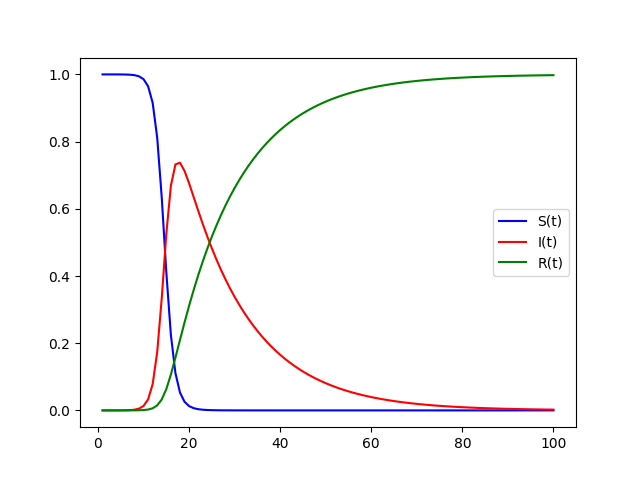
\includegraphics[width=\linewidth]{./assets/sir-graph.png}
        \label{fig:sir-chart}
        \caption{\scriptsize \sffamily The diagram\cite{sirGraph} of SIR model. \\ \quad($\beta=1$ and $\gamma=0.1$)}
	\end{minipage}
\end{figure}

% Methodology
\section{Methodology}

\subsection{Agent-based Model}
In order to construct an agent-based model, it is necessary to define the agents, their behaviours, the interactions between them, and the environment in which the agents operate. 
The agent-based model was implemented in TypeScript due to the author's familiarity with this programming language.
In general, agents are collections of properties, such as name, age, gender, health, and so on. They are used to represent the individuals, playing an important role in the simulation.
The behaviours of the agents in this model represent their daily routines and the locations of the agents at a specific time.

\subsection{Environment}
The term "environment" is defined as the space in which the agents reside. The dynamics of the agents can be understood as the movement of the agents within this space, which is influenced by their routines.

\subsection{Dynamics}
\subsubsection{Infection Possibility}
In order to simulate the spread of the disease, it is necessary to consider how healthy agents interact with infected agents and become infected. If infected agents move in close proximity to healthy agents, the risk of infection will be increased. A simple formula that can be used to roughly represent this is as follows.

\[
\mathbb{P}(\text{Infection})=\begin{cases}
	\dfrac{1}{d^2} &\quad \text{(for $d > 1$)} \\
	1 &\quad \text{(for $d \leq 1$)}
\end{cases}\quad\text{($d$ is the between the agents)}
\]

The graph of the above formula is shown in the figure below.

\begin{figure}[ht]
	\centering
	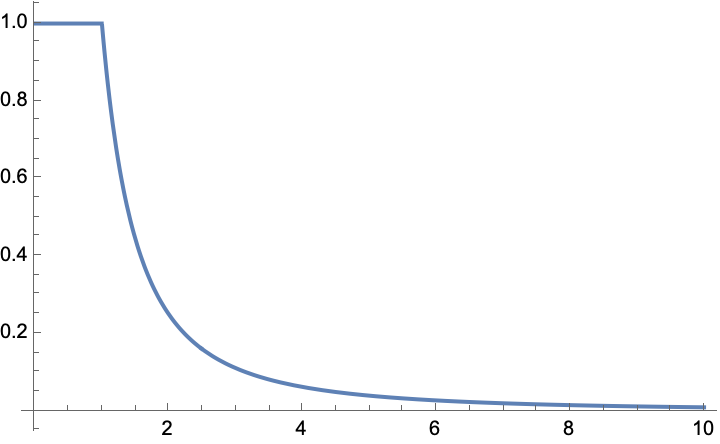
\includegraphics[width=0.55\linewidth]{./assets/infection-possibility-graph.png}
    \label{fig:infection-possibility-graph}
	\caption{The graph of possibility of infection.}
\end{figure}

Where the $x$ is the distance between the agents, calculated by the formula.

\[
d=\sqrt{(x_1-x_2)^2+(y_1-y_2)^2}
\]

Every agents will randomly get infected with a certain probability.

\subsubsection{Restoration}

Upon infection of the agents, a timer will commence a countdown. Upon reaching zero, the timer will initiate the restoration of the agents. It can be assumed that the restored agents will not become infected by the same disease.

\subsection{Implementation}

This model is implemented in TypeScript for the purpose of type safety, which enables the model to be well structured in a logical and comprehensible manner. However, the graphing of the model is implemented in R due to the availability of the powerful plotting package  \texttt{ggplot2}.

The model's graphical representation (Fig. \ref{fig:model-structure}), which illustrates the design and the manner in which the modules interact with one another, can be found in the appendix.
The flow chart of the model (Fig. \ref{fig:model-flow-chart}) is also included in the appendix.

% Results
\section{Results}
The report generated by the model is appended in the Appendix. The graphic part of the report and the parameters are shown below.

\begin{itemize}
    \item Simulation Time: 60
    \item Agent Number: 40
    \item Room Size: 40
\end{itemize}

\leftline{The disease which in this simulation model:}

\begin{itemize}
	\item Disease Name: Cold
	\item Disease Severity: 100
	\item Disease Time to Restore: 10
\end{itemize}

\begin{figure}[ht]
	\centering
	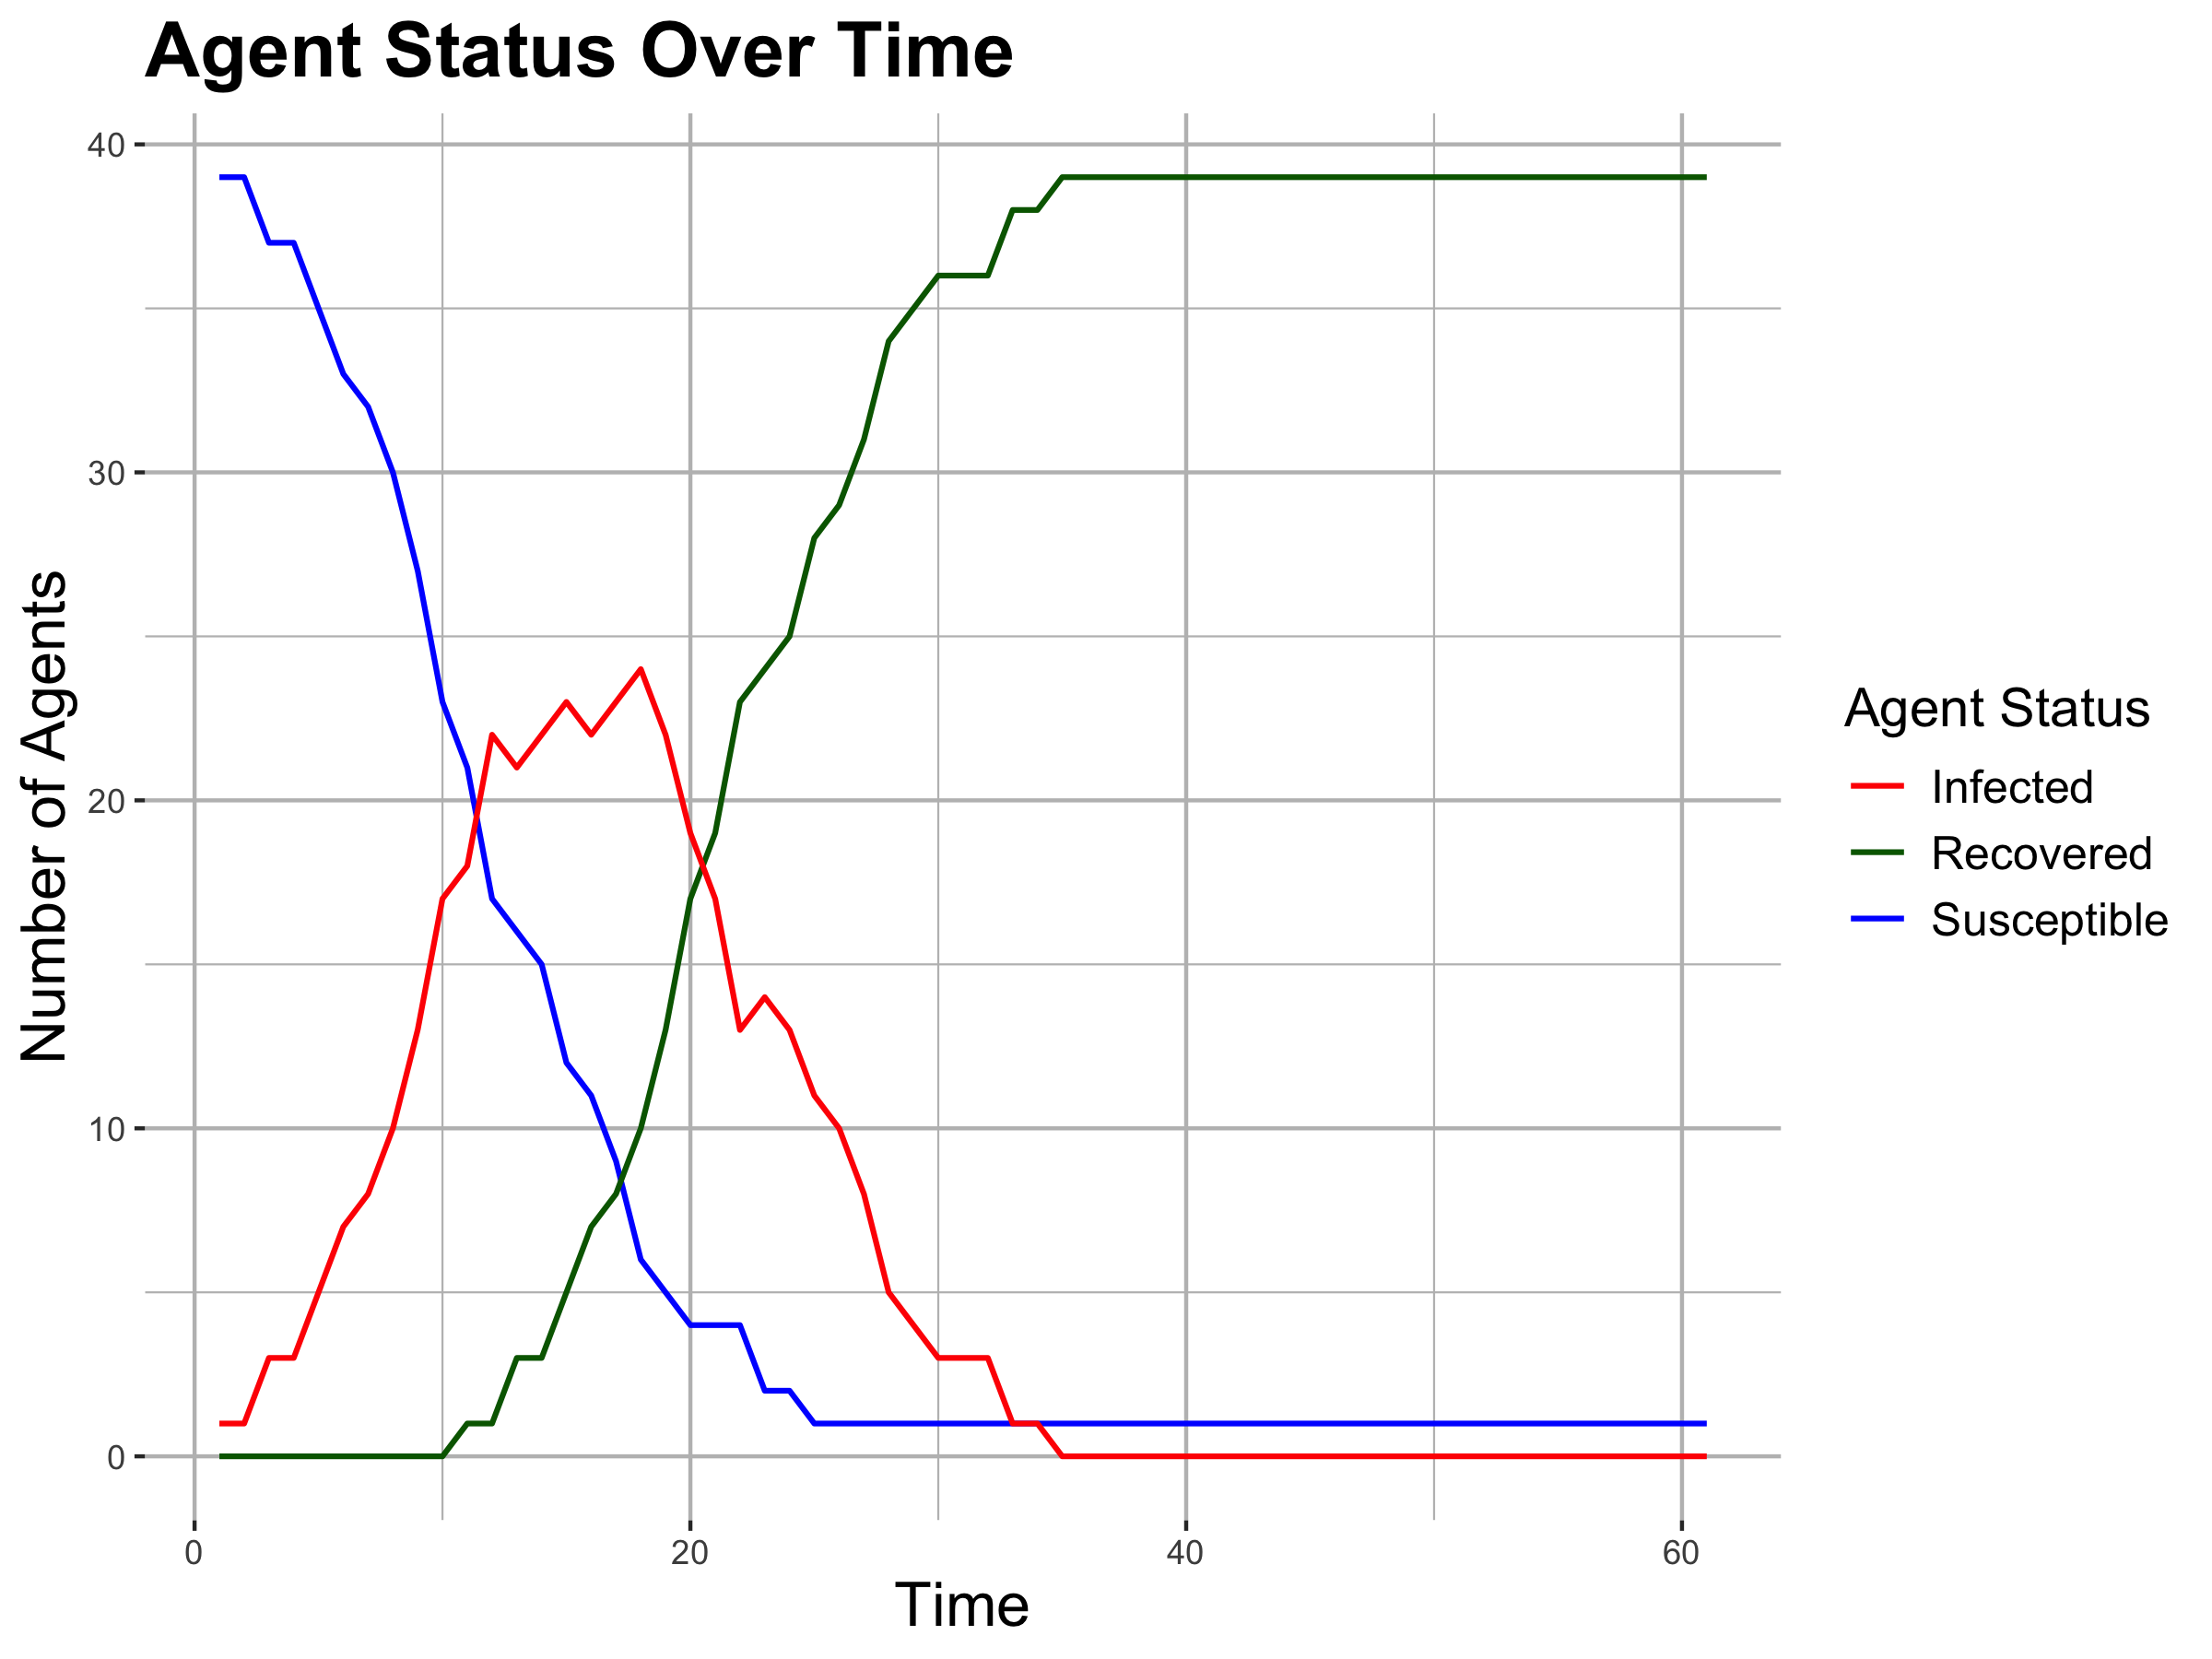
\includegraphics[width=0.9\linewidth]{./assets/report-20246030-132911/diagram.png}
    \label{fig:agent-based-model-chart} 
	\caption{\scriptsize \sffamily The diagram of the created agent-based model}
\end{figure}

It is evident that this model is capable of partially simulating the spread of the disease with given parameters in relation to the agents and diseases, due to the similarity between the previous figures (Fig.\ref{fig:sir-chart}) and this figure (Fig.\ref{fig:agent-based-model-chart}), which depict outbreaks and extinctions.

% Discussion
\section{Discussion}
This model is an effective tool for simulating the simple spread of the disease. It has been developed in TypeScript, a language chosen for its maintainability, but it lacks the ability to simulate the multiple diseases with complex dynamics. Some features that could facilitate the migration and control of parameters such as $\beta$ and $\gamma$ are missing and should be added in the future. And this model use recover time to simulate, not the possibility to recover for the agents. The author has chosen to write in TypeScript, a language that is not commonly used for data analysis, due to its familiarity. This model also lacks simulation for some complex mechanisms between the infection possibility and the age, health of the agents, the severity of the disease, etc.

% Conclusion
\section{Conclusion}
The model described above is capable of accurately simulating the spread of the disease, including the occurrence of outbreaks and extinctions.

% References
\section{References}
\printbibliography[heading=none]

\newpage

\section{Appendix}
\begin{appendices}
    \subsection{The test run report for the model}
    \leftline{The content of the report can be found in the following URL (\texttt{JSON} format)}
    \url{https://pastecode.io/s/twvh8go9}

    \subsection{The structrue of the agent-based model}
    \begin{figure}[ht]
		\centering
		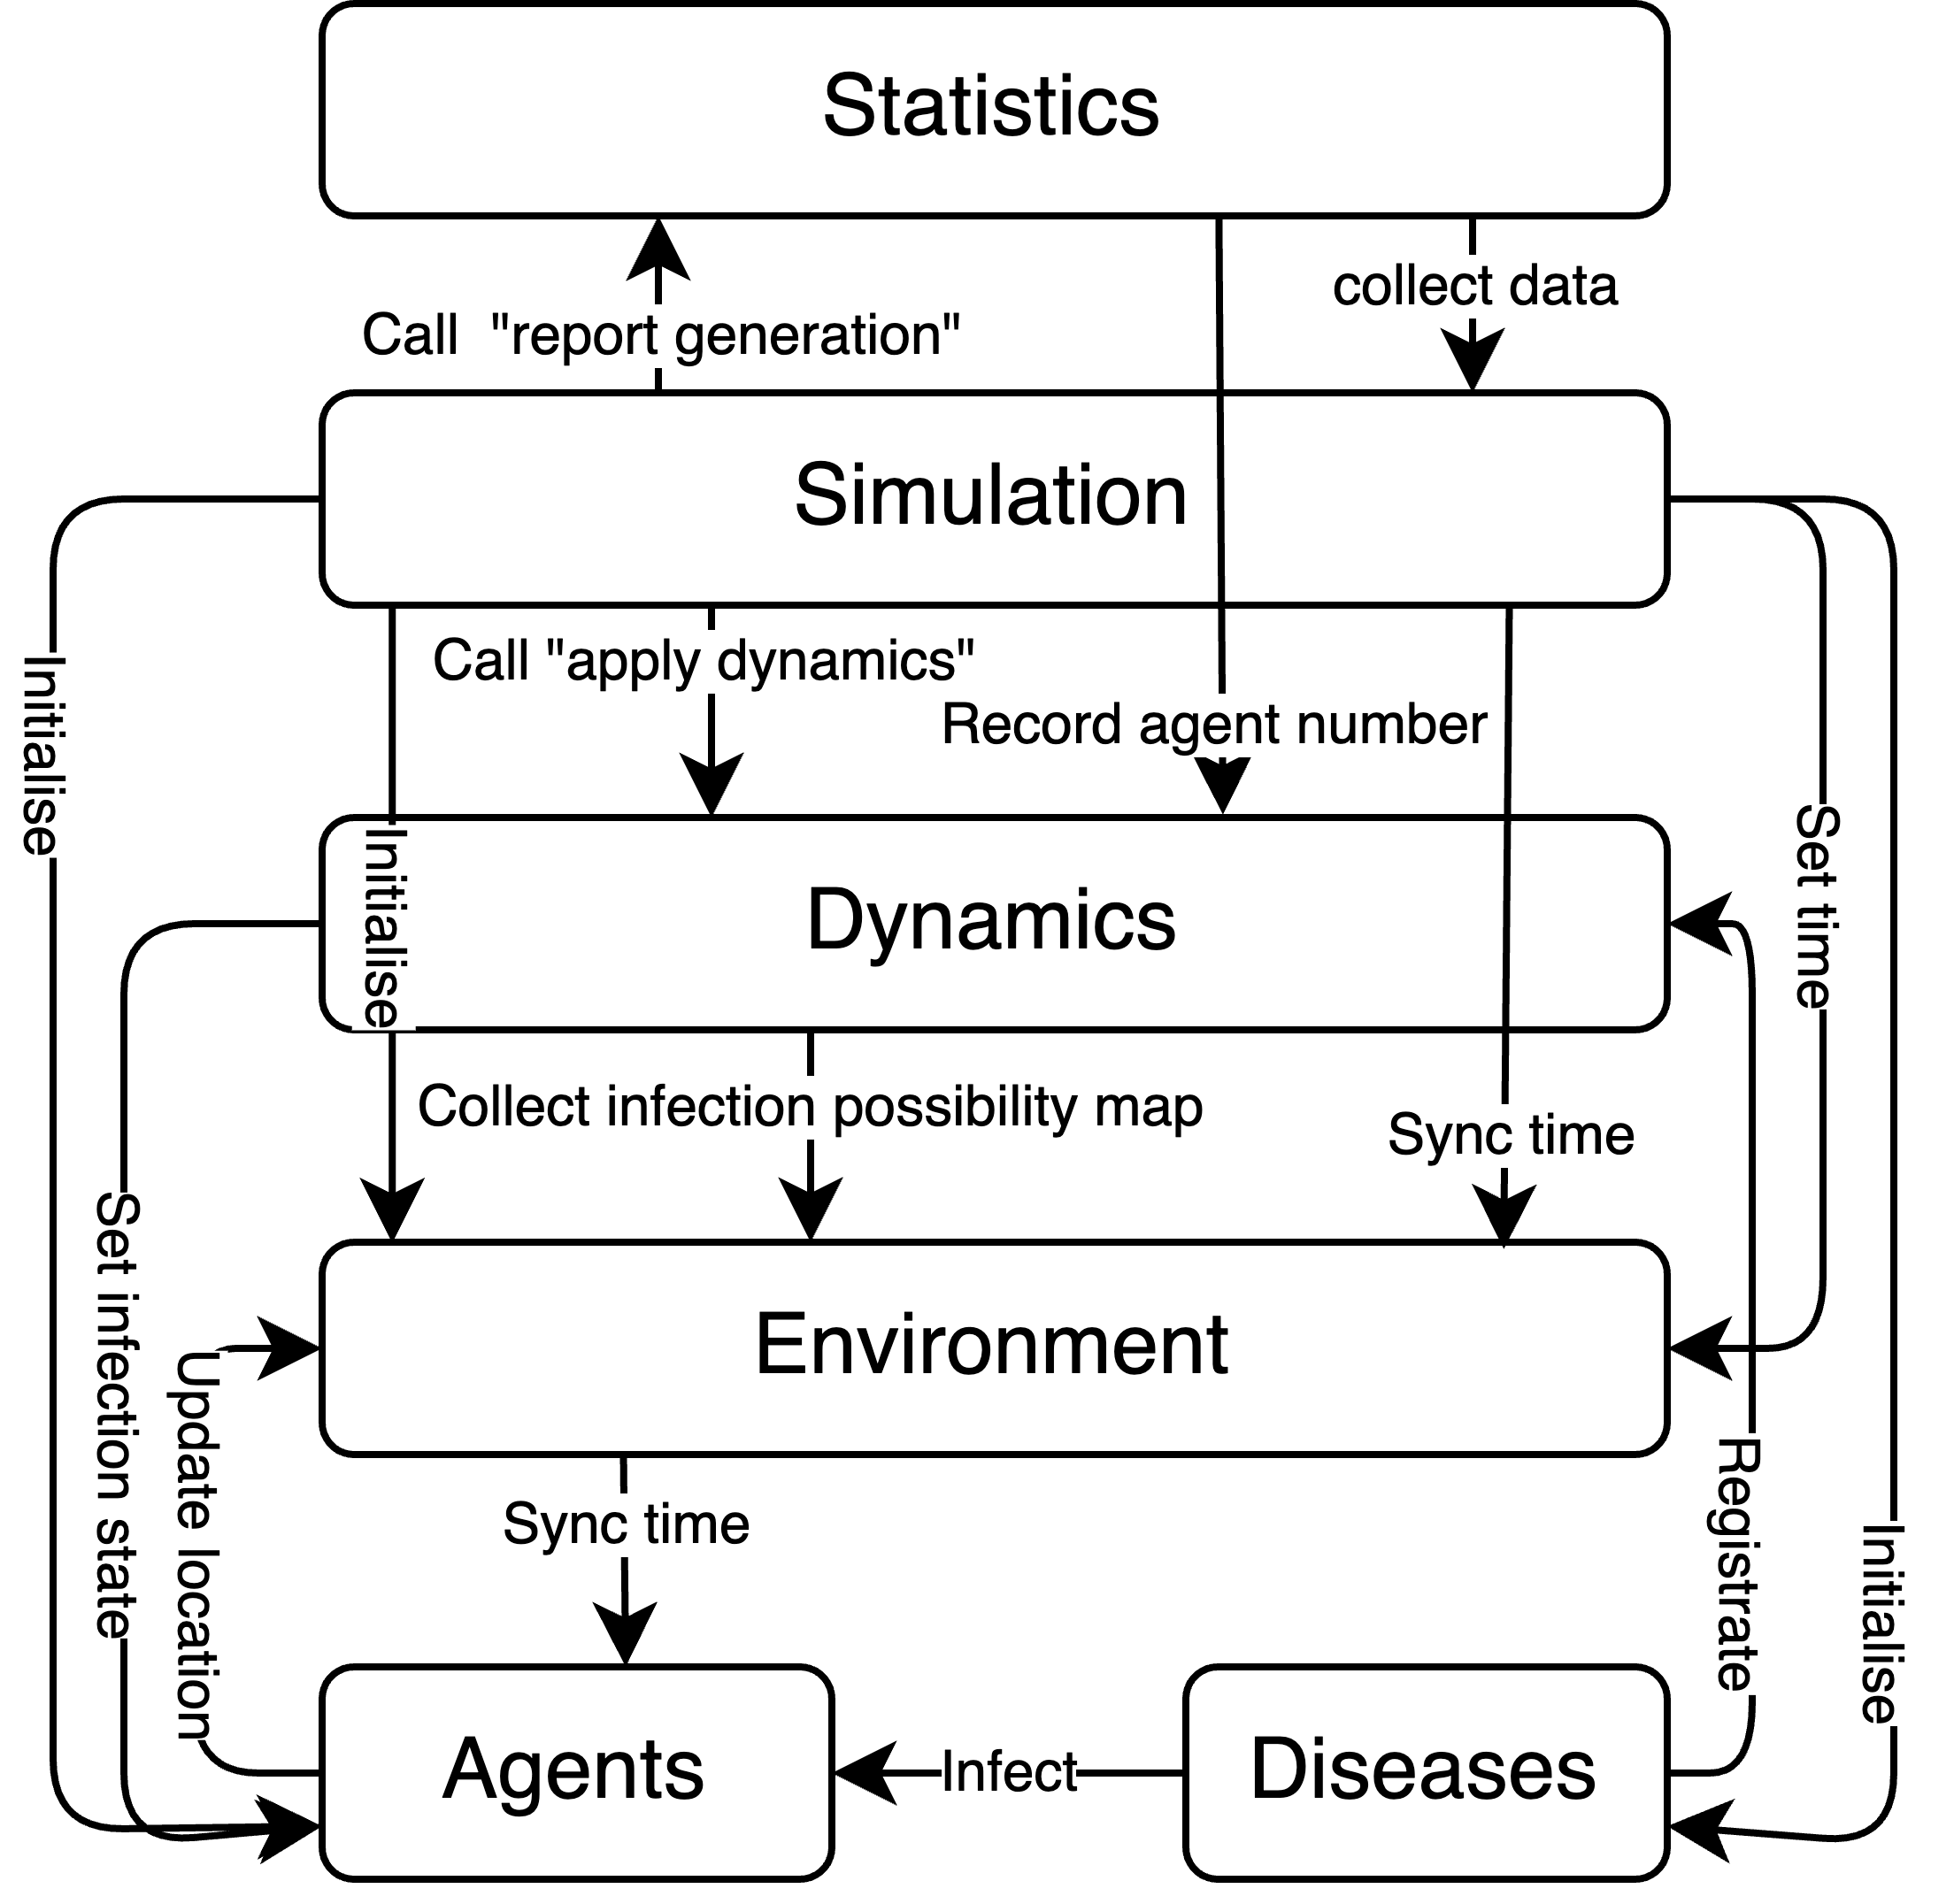
\includegraphics[width=0.6\linewidth]{./assets/model-structure.png}
        \label{fig:model-structure}
		\caption{\scriptsize \sffamily The structure of the created agent-based model} 
	\end{figure}

    \newpage

	\subsection{The flow chart of the agent-based model}
	\begin{figure}[ht]
		\centering
		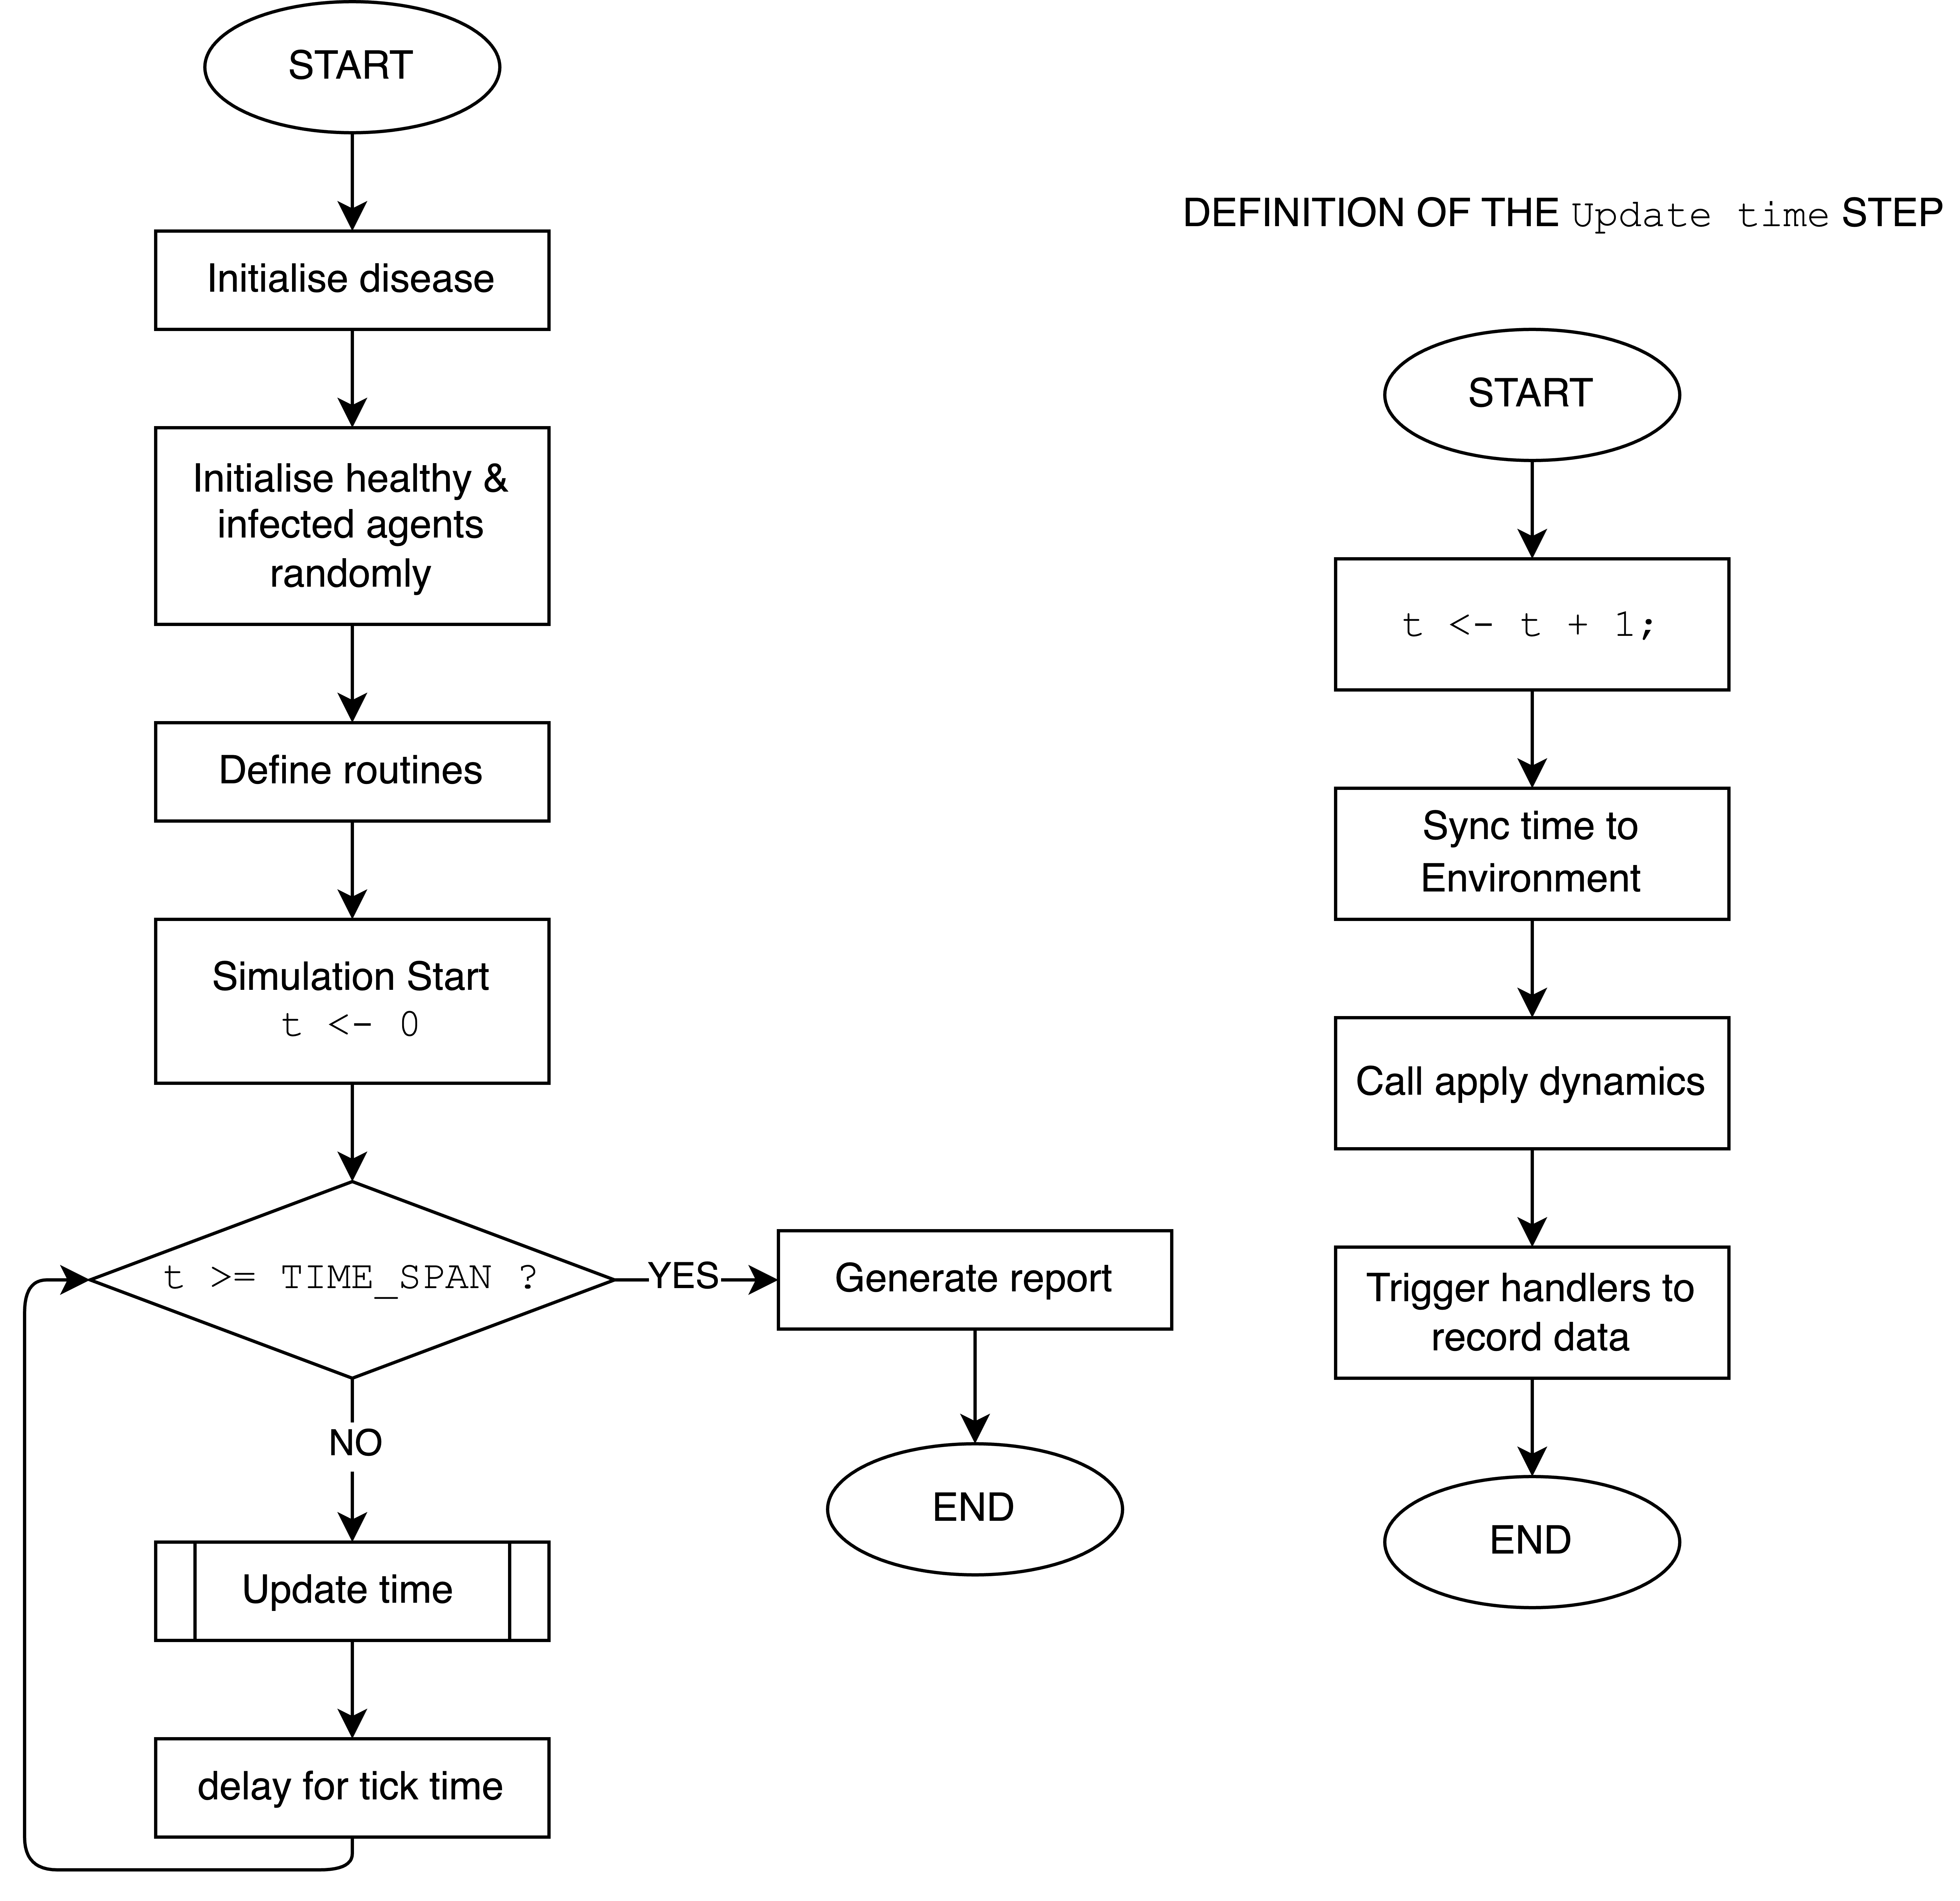
\includegraphics[width=\linewidth]{./assets/model-flow-chart.png}
        \label{fig:model-flow-chart} 
		\caption{\scriptsize \sffamily The flow chart of the created agent-based model}
	\end{figure}
\end{appendices}

\end{document}